\section{TfeTextView class}\label{tfetextview-class}

The TfeTextView class will be finally completed in this section. The
remaining topic is functions. TfeTextView functions, which are
constructors and instance methods, are described in this section.

The source files are in the directory
\passthrough{\lstinline!src/tfetextview!}. You can get them by
downloading the
\href{https://github.com/ToshioCP/Gtk4-tutorial}{repository}.

\subsection{tfetextview.h}\label{tfetextview.h}

The header file \passthrough{\lstinline!tfetextview.h!} provides:

\begin{itemize}
\tightlist
\item
  The type of TfeTextView, which is
  \passthrough{\lstinline!TFE\_TYPE\_TEXT\_VIEW!}.
\item
  The macro \passthrough{\lstinline!G\_DECLARE\_FINAL\_TYPE!}, the
  expansion of which includes some useful functions and definitions.
\item
  Constants for the \passthrough{\lstinline!open-response!} signal.
\item
  Public functions of \passthrough{\lstinline!tfetextview.c!}. They are
  constructors and instance methods.
\end{itemize}

Therefore, Any programs use TfeTextView needs to include
\passthrough{\lstinline!tfetextview.h!}.

\begin{lstlisting}[language=C, numbers=left]
#pragma once

#include <gtk/gtk.h>

#define TFE_TYPE_TEXT_VIEW tfe_text_view_get_type ()
G_DECLARE_FINAL_TYPE (TfeTextView, tfe_text_view, TFE, TEXT_VIEW, GtkTextView)

/* "open-response" signal response */
enum TfeTextViewOpenResponseType
{
  TFE_OPEN_RESPONSE_SUCCESS,
  TFE_OPEN_RESPONSE_CANCEL,
  TFE_OPEN_RESPONSE_ERROR
};

GFile *
tfe_text_view_get_file (TfeTextView *tv);

void
tfe_text_view_open (TfeTextView *tv, GtkWindow *win);

void
tfe_text_view_save (TfeTextView *tv);

void
tfe_text_view_saveas (TfeTextView *tv);

GtkWidget *
tfe_text_view_new_with_file (GFile *file);

GtkWidget *
tfe_text_view_new (void);
\end{lstlisting}

\begin{itemize}
\tightlist
\item
  1: The preprocessor directive \passthrough{\lstinline!\#pragma once!}
  makes the header file be included only once. It is non-standard but
  widely used.
\item
  3: Includes gtk4 header files. The header file
  \passthrough{\lstinline!gtk4!} also has the same mechanism to avoid
  being included multiple times.
\item
  5-6: These two lines define TfeTextView type, its class structure and
  some useful definitions.

  \begin{itemize}
  \tightlist
  \item
    \passthrough{\lstinline!TfeTextView!} and
    \passthrough{\lstinline!TfeTextViewClass!} are declared as typedef
    of C structures.
  \item
    You need to define a structure
    \passthrough{\lstinline!\_TfeTextView!} later.
  \item
    The class structure \passthrough{\lstinline!\_TfeTextViewClass!} is
    defined here. You don't need to define it by yourself.
  \item
    Convenience functions \passthrough{\lstinline!TFE\_TEXT\_VIEW ()!}
    for casting and \passthrough{\lstinline!TFE\_IS\_TEXT\_VIEW!} for
    type check are defined.
  \end{itemize}
\item
  8-14: A definition of the values of the ``open-response'' signal
  parameters.
\item
  16-32: Declarations of public functions on TfeTextView.
\end{itemize}

\subsection{Constructors}\label{constructors}

A TfeTextView instance is created with
\passthrough{\lstinline!tfe\_text\_view\_new!} or
\passthrough{\lstinline!tfe\_text\_view\_new\_with\_file!}. These
functions are called constructors.

\begin{lstlisting}[language=C]
GtkWidget *tfe_text_view_new (void);
\end{lstlisting}

It just creates a new TfeTextView instance and returns the pointer to
the new instance.

\begin{lstlisting}[language=C]
GtkWidget *tfe_text_view_new_with_file (GFile *file);
\end{lstlisting}

It is given a Gfile object as an argument and it loads the file into the
GtkTextBuffer instance, then returns the pointer to the new instance.
The argument \passthrough{\lstinline!file!} is owned by the caller and
the function doesn't change it. If an error occurs during the creation
process, NULL will be returned.

Each function is defined as follows.

\begin{lstlisting}[language=C, numbers=left]
GtkWidget *
tfe_text_view_new_with_file (GFile *file) {
  g_return_val_if_fail (G_IS_FILE (file), NULL);

  GtkWidget *tv;
  GtkTextBuffer *tb;
  char *contents;
  gsize length;

  if (! g_file_load_contents (file, NULL, &contents, &length, NULL, NULL)) /* read error */
    return NULL;

  tv = tfe_text_view_new();
  tb = gtk_text_view_get_buffer (GTK_TEXT_VIEW (tv));
  gtk_text_buffer_set_text (tb, contents, length);
  TFE_TEXT_VIEW (tv)->file = g_file_dup (file);
  gtk_text_buffer_set_modified (tb, FALSE);
  g_free (contents);
  return tv;
}

GtkWidget *
tfe_text_view_new (void) {
  return GTK_WIDGET (g_object_new (TFE_TYPE_TEXT_VIEW, "wrap-mode", GTK_WRAP_WORD_CHAR, NULL));
}
\end{lstlisting}

\begin{itemize}
\tightlist
\item
  22-25: \passthrough{\lstinline!tfe\_text\_view\_new!} function. Just
  returns the value from the function
  \passthrough{\lstinline!g\_object\_new!} but casts it to the pointer
  to GtkWidget. The function \passthrough{\lstinline!g\_object\_new!}
  creates any instances of its descendant class. The arguments are the
  type of the class, property list and NULL, which is the end mark of
  the property list. TfeTextView ``wrap-mode'' property has
  GTK\_WRAP\_WORD\_CHAR as the default value.
\item
  1-20: \passthrough{\lstinline!tfe\_text\_view\_new\_with\_file!}
  function.
\item
  3: \passthrough{\lstinline!g\_return\_val\_if\_fail!} is described in
  \href{https://docs.gtk.org/glib/func.return_val_if_fail.html}{GLib API
  Reference -- g\_return\_val\_if\_fail}. And also
  \href{https://docs.gtk.org/glib/logging.html}{GLib API Reference --
  Message Logging}. It tests whether the argument
  \passthrough{\lstinline!file!} is a pointer to GFile. If it's true,
  the program goes on to the next line. If it's false, it returns NULL
  (the second argument) immediately. And at the same time it logs out
  the error message (usually the log is outputted to stderr or stdout).
  This function is used to check the programmer's error. If an error
  occurs, the solution is usually to change the (caller) program and fix
  the bug. You need to distinguish programmer's errors and runtime
  errors. You shouldn't use this function to find runtime errors.
\item
  10-11: Reads the file. If an error occurs, NULL is returned.
\item
  13: Calls the function \passthrough{\lstinline!tfe\_text\_view\_new!}.
  The function creates TfeTextView instance and returns the pointer to
  the instance.
\item
  14: Gets the pointer to the GtkTextBuffer instance corresponds to
  \passthrough{\lstinline!tv!}. The pointer is assigned to
  \passthrough{\lstinline!tb!}
\item
  15: Assigns the contents read from the file to
  \passthrough{\lstinline!tb!}.
\item
  16: Duplicates \passthrough{\lstinline!file!} and sets
  \passthrough{\lstinline!tv->file!} to point it. GFile is \emph{not}
  thread safe. The duplication makes sure that the GFile instance of
  \passthrough{\lstinline!tv!} keeps the file information even if the
  original one is changed by other thread.
\item
  17: The function
  \passthrough{\lstinline!gtk\_text\_buffer\_set\_modified (tb, FALSE)!}
  sets the modification flag of \passthrough{\lstinline!tb!} to FALSE.
  The modification flag indicates that the contents has been modified.
  It is used when the contents are saved. If the modification flag is
  FALSE, it doesn't need to save the contents.
\item
  18: Frees the memories pointed by \passthrough{\lstinline!contents!}.
\item
  19: Returns \passthrough{\lstinline!tv!}, which is a pointer to the
  newly created TfeTextView instance. If an error happens, NULL is
  returned.
\end{itemize}

\subsection{Save and saveas functions}\label{save-and-saveas-functions}

Save and saveas functions write the contents in the GtkTextBuffer to a
file.

\begin{lstlisting}[language=C]
void tfe_text_view_save (TfeTextView *tv)
\end{lstlisting}

The function \passthrough{\lstinline!tfe\_text\_view\_save!} writes the
contents in the GtkTextBuffer to a file specified by
\passthrough{\lstinline!tv->file!}. If
\passthrough{\lstinline!tv->file!} is NULL, then it shows file chooser
dialog and prompts the user to choose a file to save. Then it saves the
contents to the file and sets \passthrough{\lstinline!tv->file!} to
point the GFile instance for the file.

\begin{lstlisting}[language=C]
void tfe_text_view_saveas (TfeTextView *tv)
\end{lstlisting}

The function \passthrough{\lstinline!saveas!} shows a file chooser
dialog and prompts the user to select a existed file or specify a new
file to save. Then, the function changes
\passthrough{\lstinline!tv->file!} and save the contents to the
specified file. If an error occurs, it is shown to the user through the
alert dialog. The error is managed only in the TfeTextView and no
information is notified to the caller.

\subsubsection{save\_file function}\label{save_file-function}

\begin{lstlisting}[language=C, numbers=left]
static gboolean
save_file (GFile *file, GtkTextBuffer *tb, GtkWindow *win) {
  GtkTextIter start_iter;
  GtkTextIter end_iter;
  char *contents;
  gboolean stat;
  GtkAlertDialog *alert_dialog;
  GError *err = NULL;

  gtk_text_buffer_get_bounds (tb, &start_iter, &end_iter);
  contents = gtk_text_buffer_get_text (tb, &start_iter, &end_iter, FALSE);
  stat = g_file_replace_contents (file, contents, strlen (contents), NULL, TRUE, G_FILE_CREATE_NONE, NULL, NULL, &err);
  if (stat)
    gtk_text_buffer_set_modified (tb, FALSE);
  else {
    alert_dialog = gtk_alert_dialog_new ("%s", err->message);
    gtk_alert_dialog_show (alert_dialog, win);
    g_object_unref (alert_dialog);
    g_error_free (err);
  }
  g_free (contents);
  return stat;
}
\end{lstlisting}

\begin{itemize}
\tightlist
\item
  The function \passthrough{\lstinline!save\_file!} is called from
  \passthrough{\lstinline!saveas\_dialog\_response!} and
  \passthrough{\lstinline!tfe\_text\_view\_save!}. This function saves
  the contents of the buffer to the file given as an argument. If error
  happens, it displays an error message. So, a caller of this function
  don't need to take care of errors. The class of this function is
  \passthrough{\lstinline!static!}. Therefore, only functions in this
  file (\passthrough{\lstinline!tfetextview.c!}) call this function.
  Such static functions usually don't have
  \passthrough{\lstinline!g\_return\_val\_if\_fail!} functions.
\item
  10-11: Gets the text contents from the buffer.
\item
  12: The function \passthrough{\lstinline!g\_file\_replace\_contents!}
  writes the contents to the file and returns the status (true =
  success/ false = fail). It has many parameters, but some of them are
  almost always given the same values.

  \begin{itemize}
  \tightlist
  \item
    GFile* file: GFile to which the contents are saved.
  \item
    const char* contents: contents to be saved. The string is owned by
    the caller.
  \item
    gsize length: the length of the contents
  \item
    const char* etag: entity tag. It is usually NULL.
  \item
    gboolean make\_backup: true to make a backup if the file exists.
    false not to make it. the file will be overwritten.
  \item
    GFileCreateFlags flags: usually
    \passthrough{\lstinline!G\_FILE\_CREATE\_NONE!} is fine.
  \item
    char** new\_etag: new entity tag. It is usually NULL.
  \item
    GCancellable* cancellable: If a cancellable instance is set, the
    other thread can cancel this operation. it is usually NULL.
  \item
    GError** error: If error happens, GError will be set.
  \end{itemize}
\item
  13,14: If no error happens, set the modified flag to be FALSE. This
  means that the buffer is not modified since it has been saved.
\item
  16-19: If it fails to save the contents, an error message will be
  displayed.
\item
  16: Creates an alert dialog. The parameters are printf-like format
  string followed by values to insert into the string. GtkAlertDialog is
  available since version 4.10. If your version is older than 4.10, use
  GtkMessageDialog instead. GtkMessageDialog is deprecated since version
  4.10.
\item
  17: Show the alert dialog. The parameters are the dialog and the
  transient parent window. This allows window managers to keep the
  dialog on top of the parent window, or center the dialog over the
  parent window. It is possible to give no parent window to the dialog
  by giving NULL as the argument. However, it is encouraged to give
  parents to dialogs.
\item
  18: Releases the dialog.
\item
  19: Frees the GError struct pointed by \passthrough{\lstinline!err!}
  with \passthrough{\lstinline!g\_error\_free!} function.
\item
  21: Frees \passthrough{\lstinline!contents!}.
\item
  22: Returns the status to the caller.
\end{itemize}

\subsubsection{save\_dialog\_cb function}\label{save_dialog_cb-function}

\begin{lstlisting}[language=C, numbers=left]
static void
save_dialog_cb(GObject *source_object, GAsyncResult *res, gpointer data) {
  GtkFileDialog *dialog = GTK_FILE_DIALOG (source_object);
  TfeTextView *tv = TFE_TEXT_VIEW (data);
  GtkTextBuffer *tb = gtk_text_view_get_buffer (GTK_TEXT_VIEW (tv));
  GFile *file;
  GtkWidget *win = gtk_widget_get_ancestor (GTK_WIDGET (tv), GTK_TYPE_WINDOW);
  GError *err = NULL;
  GtkAlertDialog *alert_dialog;

  if (((file = gtk_file_dialog_save_finish (dialog, res, &err)) != NULL) && save_file(file, tb, GTK_WINDOW (win))) {
    // The following is complicated. The comments here will help your understanding
    // G_IS_FILE(tv->file) && tv->file == file  => nothing to do
    // G_IS_FILE(tv->file) && tv->file != file  => unref(tv->file), tv->file=file, emit change_file signal
    // tv->file==NULL                           =>                  tv->file=file, emit change_file signal
    if (! (G_IS_FILE (tv->file) && g_file_equal (tv->file, file))) {
      if (G_IS_FILE (tv->file))
        g_object_unref (tv->file);
      tv->file = file; // The ownership of 'file' moves to TfeTextView.
      g_signal_emit (tv, tfe_text_view_signals[CHANGE_FILE], 0);
    }
  }
  if (err) {
    alert_dialog = gtk_alert_dialog_new ("%s", err->message);
    gtk_alert_dialog_show (alert_dialog, GTK_WINDOW (win));
    g_object_unref (alert_dialog);
    g_clear_error (&err);
  }
}
\end{lstlisting}

\begin{itemize}
\tightlist
\item
  The function \passthrough{\lstinline!save\_dialog\_cb!} is a call back
  function that is given to the
  \passthrough{\lstinline!gtk\_file\_dialog\_save!} function as an
  argument. The \passthrough{\lstinline!gtk\_file\_dialog\_save!} shows
  a file chooser dialog to the user. The user chooses or types a
  filename and clicks on the \passthrough{\lstinline!Save!} button or
  just clicks on the \passthrough{\lstinline!Cancel!} button. Then the
  call back function is called with the result. This is the general way
  in GIO to manage asynchronous operations. A pair of functions
  \passthrough{\lstinline!g\_data\_input\_stream\_read\_line\_async!}
  and
  \passthrough{\lstinline!g\_data\_input\_stream\_read\_line\_finish!}
  are one example. These functions are thread-safe. The arguments of
  \passthrough{\lstinline!save\_dialog\_cb!} are:

  \begin{itemize}
  \tightlist
  \item
    GObject *source\_object: The GObject instance that the operation was
    started with. It is actually the GtkFileDialog instance that is
    shown to the user. However, the call back function is defined as
    \passthrough{\lstinline!AsyncReadyCallback!}, which is a general
    call back function for an asynchronous operation. So the type is
    GObject and you need to cast it to GtkFileDialog later.
  \item
    GAsyncResult *res: The result of the asynchronous operation. It will
    be given to the \passthrough{\lstinline!gtk\_dialog\_save\_finish!}
    function.
  \item
    gpointer data: A user data set in the
    \passthrough{\lstinline!gtk\_dialog\_save!} function.
  \end{itemize}
\item
  11: Calls \passthrough{\lstinline!gtk\_dialog\_save\_finish!}. It is
  given the result \passthrough{\lstinline!res!} as an argument and
  returns a pointer to a GFile object the user has chosen. If the user
  has canceled or an error happens, it returns NULL, creates a GError
  object and sets \passthrough{\lstinline!err!} to point it. If
  \passthrough{\lstinline!gtk\_dialog\_save\_finish!} returns a GFile,
  the function \passthrough{\lstinline!save\_file!} is called.
\item
  12-21: If the file is successfully saved, these lines are executed.
  See the comments, line 12-15, for the details.
\item
  23-28: If an error happens, show the error message through the alert
  dialog.
\end{itemize}

\subsubsection{tfe\_text\_view\_save
function}\label{tfe_text_view_save-function}

\begin{lstlisting}[language=C, numbers=left]
void
tfe_text_view_save (TfeTextView *tv) {
  g_return_if_fail (TFE_IS_TEXT_VIEW (tv));

  GtkTextBuffer *tb = gtk_text_view_get_buffer (GTK_TEXT_VIEW (tv));
  GtkWidget *win = gtk_widget_get_ancestor (GTK_WIDGET (tv), GTK_TYPE_WINDOW);

  if (! gtk_text_buffer_get_modified (tb))
    return; /* no need to save it */
  else if (tv->file == NULL)
    tfe_text_view_saveas (tv);
  else
    save_file (tv->file, tb, GTK_WINDOW (win));
}
\end{lstlisting}

\begin{itemize}
\tightlist
\item
  The function \passthrough{\lstinline!tfe\_text\_view\_save!} writes
  the contents to the \passthrough{\lstinline!tv->file!} file. It calls
  \passthrough{\lstinline!tfe\_text\_view\_saveas!} or
  \passthrough{\lstinline!save\_file!}.
\item
  1-3: The function is public, i.e.~it is open to the other objects. So,
  it doesn't have \passthrough{\lstinline!static!} class. Public
  functions should check the parameter type with
  \passthrough{\lstinline!g\_return\_if\_fail!} function. If
  \passthrough{\lstinline!tv!} is not a pointer to a TfeTextView
  instance, then it logs an error message and immediately returns. This
  function is similar to
  \passthrough{\lstinline!g\_return\_val\_if\_fail!}, but no value is
  returned because \passthrough{\lstinline!tfe\_text\_view\_save!}
  doesn't return a value (void).
\item
  5-6: GtkTextBuffer \passthrough{\lstinline!tb!} and GtkWidget
  (GtkWindow) \passthrough{\lstinline!win!} are set. The function
  \passthrough{\lstinline!gtk\_widget\_get\_ancestor (widget, type)!}
  returns the first ancestor of the widget with the type, which is a
  GType. The parent-child relationship here is the one for widgets, not
  classes. More precisely, the returned widget's type is the
  \passthrough{\lstinline!type!} or a descendant object type of the
  \passthrough{\lstinline!type!}. Be careful, the ``descendant object''
  in the previous sentence is \emph{not} ``descendant widget''. For
  example, the type of GtkWindow is
  \passthrough{\lstinline!GTK\_TYPE\_WINDOW!} and the one of TfeTextView
  is \passthrough{\lstinline!TFE\_TYPE\_TEXT\_VIEW!}. The top level
  window may be a GtkApplicationWindow, but it is a descendant of
  GtkWindow. Therefore,
  \passthrough{\lstinline!gtk\_widget\_get\_ancestor (GTK\_WIDGET (tv), GTK\_TYPE\_WINDOW)!}
  possibly returns GtkWindow or GtkApplicationWindow.
\item
  8-9: If the buffer hasn't modified, it doesn't need to be saved.
\item
  10-11: If \passthrough{\lstinline!tv->file!} is NULL, which means no
  file has given yet, it calls
  \passthrough{\lstinline!tfe\_text\_view\_saveas!} to prompt a user to
  select a file and save the contents.
\item
  12-13: Otherwise, it calls \passthrough{\lstinline!save\_file!} to
  save the contents to the file \passthrough{\lstinline!tv->file!}.
\end{itemize}

\subsubsection{tfe\_text\_view\_saveas
function}\label{tfe_text_view_saveas-function}

\begin{lstlisting}[language=C, numbers=left]
void
tfe_text_view_saveas (TfeTextView *tv) {
  g_return_if_fail (TFE_IS_TEXT_VIEW (tv));

  GtkWidget *win = gtk_widget_get_ancestor (GTK_WIDGET (tv), GTK_TYPE_WINDOW);
  GtkFileDialog *dialog;

  dialog = gtk_file_dialog_new ();
  gtk_file_dialog_save (dialog, GTK_WINDOW (win), NULL, save_dialog_cb, tv);
  g_object_unref (dialog);
}
\end{lstlisting}

The function \passthrough{\lstinline!tfe\_text\_view\_saveas!} shows a
file chooser dialog and prompts the user to choose a file and save the
contents.

\begin{itemize}
\tightlist
\item
  1-3: Check the type of \passthrough{\lstinline!tv!} because the
  function is public.
\item
  6: GtkWidget \passthrough{\lstinline!win!} is set to the window which
  is an ancestor ot \passthrough{\lstinline!tv!}.
\item
  8: Creates a GtkFileDialog instance. GtkFileDialog is available since
  version 4.10. If your Gtk version is older than 4.10, use
  GtkFileChooserDialog instead. GtkFileChooserDialog is deprecated since
  version 4.10.
\item
  9: Calls \passthrough{\lstinline!gtk\_file\_dialog\_save!} function.
  The arguments are:

  \begin{itemize}
  \tightlist
  \item
    dialog: GtkFileDialog.
  \item
    GTK\_WINDOW (win): transient parent window.
  \item
    NULL: NULL means no cancellable object. If you put a cancellable
    object here, you can cancel the operation by other thread. In many
    cases, it is NULL. See
    \href{https://docs.gtk.org/gio/class.Cancellable.html}{GCancellable}
    for further information.
  \item
    \passthrough{\lstinline!save\_dialog\_cb!}: A callback to call when
    the operation is complete. The type of the pointer to the callback
    function is
    \href{https://docs.gtk.org/gio/callback.AsyncReadyCallback.html}{GAsyncReadyCallback}.
    If a cancellable object is given and the operation is cancelled, the
    callback won't be called.
  \item
    \passthrough{\lstinline!tv!}: This is an optional user data which is
    gpointer type. It is used in the callback function.
  \end{itemize}
\item
  10: Releases the GtkFileDialog instance because it is useless anymore.
\end{itemize}

This function just shows the file chooser dialog. The rest of the
operation is done by the callback function.

\begin{figure}
\centering
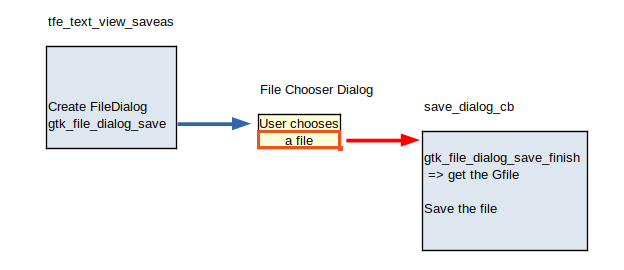
\includegraphics[width=10.7cm,height=5.16cm]{../image/saveas.png}
\caption{Saveas process}
\end{figure}

\subsection{Open related functions}\label{open-related-functions}

Open function shows a file chooser dialog to a user and prompts them to
choose a file. Then it reads the file and puts the text into
GtkTextBuffer.

\begin{lstlisting}[language=C]
void tfe_text_view_open (TfeTextView *tv, GtkWindow *win);
\end{lstlisting}

The parameter \passthrough{\lstinline!win!} is the transient window. A
file chooser dialog will be shown at the center of the window.

This function may be called just after \passthrough{\lstinline!tv!} has
been created. In that case, \passthrough{\lstinline!tv!} has not been
incorporated into the widget hierarchy. Therefore it is impossible to
get the top-level window from \passthrough{\lstinline!tv!}. That's why
the function needs \passthrough{\lstinline!win!} parameter.

This function is usually called when the buffer of
\passthrough{\lstinline!tv!} is empty. However, even if the buffer is
not empty, \passthrough{\lstinline!tfe\_text\_view\_open!} doesn't treat
it as an error. If you want to revert the buffer, calling this function
is appropriate.

Open and read process is divided into two phases. One is creating and
showing a file chooser dialog and the other is the callback function.
The former is \passthrough{\lstinline!tfe\_text\_view\_open!} and the
latter is \passthrough{\lstinline!open\_dialog\_cb!}.

\subsubsection{open\_dialog\_cb function}\label{open_dialog_cb-function}

\begin{lstlisting}[language=C, numbers=left]
static void
open_dialog_cb (GObject *source_object, GAsyncResult *res, gpointer data) {
  GtkFileDialog *dialog = GTK_FILE_DIALOG (source_object);
  TfeTextView *tv = TFE_TEXT_VIEW (data);
  GtkTextBuffer *tb = gtk_text_view_get_buffer (GTK_TEXT_VIEW (tv));
  GtkWidget *win = gtk_widget_get_ancestor (GTK_WIDGET (tv), GTK_TYPE_WINDOW);
  GFile *file;
  char *contents;
  gsize length;
  gboolean file_changed;
  GtkAlertDialog *alert_dialog;
  GError *err = NULL;

  if ((file = gtk_file_dialog_open_finish (dialog, res, &err)) != NULL
      && g_file_load_contents (file, NULL, &contents, &length, NULL, &err)) {
    gtk_text_buffer_set_text (tb, contents, length);
    g_free (contents);
    gtk_text_buffer_set_modified (tb, FALSE);
    // G_IS_FILE(tv->file) && tv->file == file => unref(tv->file), tv->file=file, emit response with SUCCESS
    // G_IS_FILE(tv->file) && tv->file != file => unref(tv->file), tv->file=file, emit response with SUCCESS, emit change-file
    // tv->file==NULL =>                                           tv->file=file, emit response with SUCCESS, emit change-file
    // The order is important. If you unref tv->file first, you can't compare tv->file and file anymore.
    // And the signals are emitted after new tv->file is set. Or the handler can't catch the new file.
    file_changed = (G_IS_FILE (tv->file) && g_file_equal (tv->file, file)) ? FALSE : TRUE;
    if (G_IS_FILE (tv->file))
      g_object_unref (tv->file);
    tv->file = file; // The ownership of 'file' moves to TfeTextView
    if (file_changed)
      g_signal_emit (tv, tfe_text_view_signals[CHANGE_FILE], 0);
    g_signal_emit (tv, tfe_text_view_signals[OPEN_RESPONSE], 0, TFE_OPEN_RESPONSE_SUCCESS);
  } else {
    if (err->code == GTK_DIALOG_ERROR_DISMISSED) // The user canceled the file chooser dialog
      g_signal_emit (tv, tfe_text_view_signals[OPEN_RESPONSE], 0, TFE_OPEN_RESPONSE_CANCEL);
    else {
      alert_dialog = gtk_alert_dialog_new ("%s", err->message);
      gtk_alert_dialog_show (alert_dialog, GTK_WINDOW (win));
      g_object_unref (alert_dialog);
      g_signal_emit (tv, tfe_text_view_signals[OPEN_RESPONSE], 0, TFE_OPEN_RESPONSE_ERROR);
    }
    g_clear_error (&err);
  }
}
\end{lstlisting}

This function is similar to \passthrough{\lstinline!save\_dialog\_cb!}.
Both are callback functions on a GtkFileDialog object.

\begin{itemize}
\tightlist
\item
  2: It has three parameters like
  \passthrough{\lstinline!save\_dialog\_cb!}. They are:

  \begin{itemize}
  \tightlist
  \item
    GObject *source\_object: The GObject instance that the operation was
    started with. It is actually the GtkFileDialog instance that is
    shown to the user. It will be casted to GtkFileDialog later.
  \item
    GAsyncResult *res: The result of the asynchronous operation. It will
    be given to the \passthrough{\lstinline!gtk\_dialog\_open\_finish!}
    function.
  \item
    gpointer data: A user data set in the
    \passthrough{\lstinline!gtk\_dialog\_open!} function. It is actually
    a TfeTextView instance and it will be casted to TfeTextView later.
  \end{itemize}
\item
  14: The function
  \passthrough{\lstinline!gtk\_file\_dialog\_open\_finish!} returns a
  GFile object if the operation has succeeded. Otherwise it returns
  NULL.
\item
  16-30: If the user selects a file and the file has successfully been
  read, the codes from 16 to 30 will be executed.
\item
  16-18: Sets the buffer of \passthrough{\lstinline!tv!} with the text
  read from the file. And frees \passthrough{\lstinline!contents!}. Then
  sets the modified status to false.
\item
  19-30: The codes are a bit complicated. See the comments. If the file
  (\passthrough{\lstinline!tv->file!}) is changed, ``change-file''
  signal is emitted. The signal ``open-response'' is emitted with the
  parameter \passthrough{\lstinline!TFE\_OPEN\_RESPONSE\_SUCCESS!}.
\item
  31-41: If the operation failed, the codes from 31 to 41 will be
  executed.
\item
  32-33: If the error code is
  \passthrough{\lstinline!GTK\_DIALOG\_ERROR\_DISMISSED!}, it means that
  the user has clicked on the ``Cancel'' button or close button on the
  header bar. Then, ``open-response'' signal is emitted with the
  parameter \passthrough{\lstinline!TFE\_OPEN\_RESPONSE\_CANCEL!}. The
  Dialog error is described
  \href{https://docs.gtk.org/gtk4/error.DialogError.html}{here} in the
  GTK API reference.
\item
  35-38: If another error occurs, it shows an alert dialog to report the
  error and emits ``open-response'' signal with the parameter
  \passthrough{\lstinline!TFE\_OPEN\_RESPONSE\_ERROR!}.
\item
  40: Clears the error structure.
\end{itemize}

\subsubsection{tfe\_text\_view\_open
function}\label{tfe_text_view_open-function}

\begin{lstlisting}[language=C, numbers=left]
void
tfe_text_view_open (TfeTextView *tv, GtkWindow *win) {
  g_return_if_fail (TFE_IS_TEXT_VIEW (tv));
  // 'win' is used for a transient window of the GtkFileDialog.
  // It can be NULL.
  g_return_if_fail (GTK_IS_WINDOW (win) || win == NULL);

  GtkFileDialog *dialog;

  dialog = gtk_file_dialog_new ();
  gtk_file_dialog_open (dialog, win, NULL, open_dialog_cb, tv);
  g_object_unref (dialog);
}
\end{lstlisting}

\begin{itemize}
\tightlist
\item
  3-6: Check the type of the arguments \passthrough{\lstinline!tv!} and
  \passthrough{\lstinline!win!}. Public functions always need to check
  the arguments.
\item
  10: Creates a GtkFileDialog instance.
\item
  11: Calls \passthrough{\lstinline!gtk\_file\_dialog\_open!}. The
  arguments are:

  \begin{itemize}
  \tightlist
  \item
    \passthrough{\lstinline!dialog!}: the GtkFileDialog instance
  \item
    \passthrough{\lstinline!win!}: the transient window for the file
    chooser dialog
  \item
    \passthrough{\lstinline!NULL!}: NULL means no cancellable object
  \item
    \passthrough{\lstinline!open\_dialog\_cb!}: callback function
  \item
    \passthrough{\lstinline!tv!}: user data which is used in the
    callback function
  \end{itemize}
\item
  12: Releases the dialog instance because it is useless anymore.
\end{itemize}

The whole process between the caller and TfeTextView is shown in the
following diagram. It is really complicated. Because
\passthrough{\lstinline!gtk\_file\_dialog\_open!} can't return the
status of the operation.

\begin{figure}
\centering
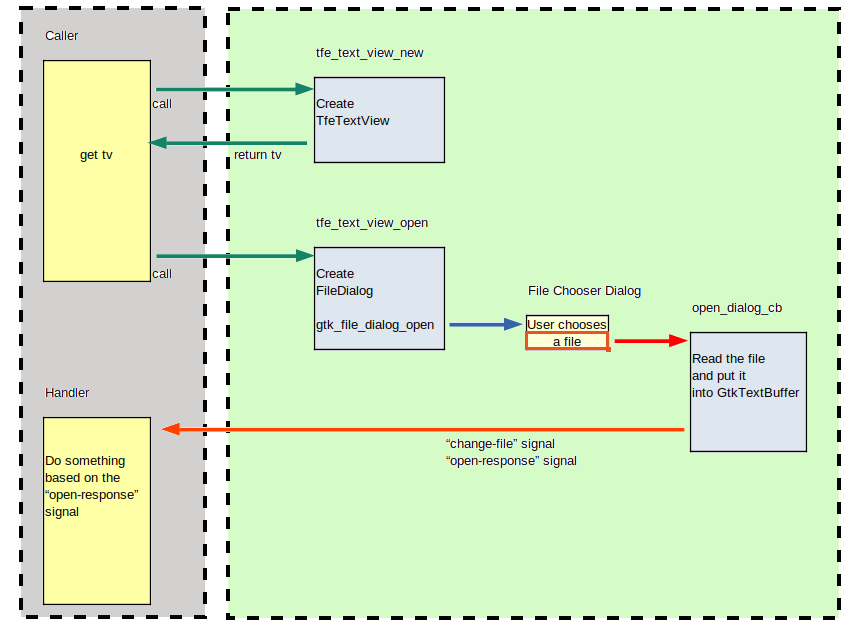
\includegraphics[width=12.405cm,height=9.225cm]{../image/open.png}
\caption{Caller and TfeTextView}
\end{figure}

\begin{enumerate}
\def\labelenumi{\arabic{enumi}.}
\tightlist
\item
  A caller gets a pointer \passthrough{\lstinline!tv!} to a TfeTextView
  instance by calling \passthrough{\lstinline!tfe\_text\_view\_new!}.
\item
  The caller connects the handler (left bottom in the diagram) and the
  signal ``open-response''.
\item
  It calls \passthrough{\lstinline!tfe\_text\_view\_open!} to prompt the
  user to select a file from the file chooser dialog.
\item
  When the dialog is closed, the callback
  \passthrough{\lstinline!open\_dialog\_cb!} is called.
\item
  The callback function reads the file and inserts the text into
  GtkTextBuffer and emits a signal to inform the status as a response
  code.
\item
  The handler of the ``open-response'' signal is invoked and the
  operation status is given to it as an argument (signal parameter).
\end{enumerate}

\subsection{Getting GFile in
TfeTextView}\label{getting-gfile-in-tfetextview}

You can get the GFile in a TfeTextView instance with
\passthrough{\lstinline!tfe\_text\_view\_get\_file!}. It is very simple.

\begin{lstlisting}[language=C, numbers=left]
GFile *
tfe_text_view_get_file (TfeTextView *tv) {
  g_return_val_if_fail (TFE_IS_TEXT_VIEW (tv), NULL);

  if (G_IS_FILE (tv->file))
    return g_file_dup (tv->file);
  else
    return NULL;
}
\end{lstlisting}

The important thing is to duplicate \passthrough{\lstinline!tv->file!}.
Otherwise, if the caller frees the GFile object,
\passthrough{\lstinline!tv->file!} is no more guaranteed to point the
GFile. Another reason to use \passthrough{\lstinline!g\_file\_dup!} is
that GFile isn't thread-safe. If you use GFile in the different thread,
the duplication is necessary. See
\href{https://docs.gtk.org/gio/method.File.dup.html}{Gio API Reference
-- g\_file\_dup}.

\subsection{The API document and source file of
tfetextview.c}\label{the-api-document-and-source-file-of-tfetextview.c}

Refer API document of TfeTextView in the appendix. The markdown file is
under the directory \passthrough{\lstinline!src/tfetextview!}.

You can find all the TfeTextView source codes under src/tfetextview
directories.
